\section{Experiment}

We conducted an experiment of our system with a Rethink Baxter robot and six wooden modules with AprilTags on them. For sensing and localization of the modules, we used the camera on Baxter's left hand and an external Kinect. In this experiment, we started from some random location of the six modules (Fig.~\ref{fig:initConfig}) and tried to form a snake configuration with the six modules (Fig.~\ref{fig:finalConfig}).
The link to a video of the experiment is \url{https://youtu.be/u-IBSN2aX7Y}. 

\begin{figure}[ht!]%[H]
\centering
\subfloat[Inital position of the modules]{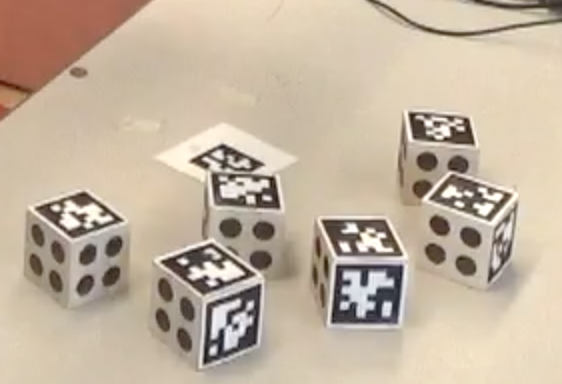
\includegraphics[width=0.45\columnwidth]{pics/init_module_location.png}\label{fig:initConfig}}
\quad
\subfloat[Final module configuration]{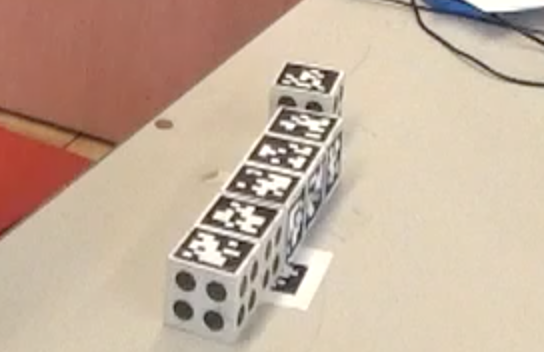
\includegraphics[width=0.45\columnwidth]{pics/snake_modules.png}\label{fig:finalConfig}}\\
\caption{Final Module Configuration}
\end{figure}

In this experiment, our system was able to recover from grasping failure and our system continued to finish the assembly with the instructions from the high-level planner. As shown in Table~\ref{table:result}, out of the five connections between the modules, our system successfully performed 3 connections: connected the third, the fourth and fifth module to the assembly. Our system failed to connect the second module to the first one due to misalignment and it also failed to connect the last module to the assembly due to too small of a motion. 


%\begin{center}
\begin{table}[h]
\caption{Connection Result of Modules} %F for Failed and S for Succeeded}
\begin{tabular}{c |c |c |c |c |c|}
\hline
 Connection &  1-2 & 2-3 & 3-4 & 4-5 & 5-6 \\\hline 
  Result  & failed & succeeded & succeeded & succeeded & failed \\\hline  
\end{tabular}\label{table:result}
\end{table}
%\end{center}

In the future, we will improve the fine adjustment to connect the modules. We will also use the right arm to localize and manipulate the modules. We plan to attempt more complex configuration to showcase the capabilities of our system.


